\let\negmedspace\undefined
\let\negthickspace\undefined
\documentclass[journal]{IEEEtran}
\usepackage[a5paper, margin=10mm, onecolumn]{geometry}
%\usepackage{lmodern} % Ensure lmodern is loaded for pdflatex
\usepackage{tfrupee} % Include tfrupee package

\setlength{\headheight}{1cm} % Set the height of the header box
\setlength{\headsep}{0mm}     % Set the distance between the header box and the top of the text

\usepackage{gvv-book}
\usepackage{gvv}
\usepackage{cite}
\usepackage{amsmath,amssymb,amsfonts,amsthm}
\usepackage{algorithmic}
\usepackage{graphicx}
\usepackage{textcomp}
\usepackage{xcolor}
\usepackage{txfonts}
\usepackage{listings}
\usepackage{enumitem}
\usepackage{mathtools}
\usepackage{gensymb}
\usepackage{comment}
\usepackage[breaklinks=true]{hyperref}
\usepackage{tkz-euclide} 
\usepackage{listings}
% \usepackage{gvv}                                        
\def\inputGnumericTable{}                                 
\usepackage[latin1]{inputenc}                                
\usepackage{color}                                            
\usepackage{array}                                            
\usepackage{longtable}                                       
\usepackage{calc}                                             
\usepackage{multirow}                                         
\usepackage{hhline}                                           
\usepackage{ifthen}                                           
\usepackage{lscape}
\begin{document}

\bibliographystyle{IEEEtran}
\vspace{3cm}

\title{5.8.10}
\author{EE25BTECH11012-BEERAM MADHURI}
% \maketitle
% \newpage
% \bigskip
{\let\newpage\relax\maketitle}

\renewcommand{\thefigure}{\theenumi}
\renewcommand{\thetable}{\theenumi}
\setlength{\intextsep}{10pt} % Space between text and floats


\numberwithin{equation}{enumi}
\numberwithin{figure}{enumi}
\renewcommand{\thetable}{\theenumi}


\textbf{Question}:\\
Narayan tells his daughter, `Seven years ago, I was seven times as old as you were then. Also, 3 years from now, I shall be 3 times as old as you will be.' Find their ages.

\textbf{Solution:}\\
Let present age of Narayan $= N$ and \\
Present age of daughter $= D$. \\
7 years ago: 
\begin{align}
(N-7) = 7(D-7) \\
N-7 = 7D -49 \\
7D-N = 42
\end{align}
and 3 years from now: 
\begin{align}
(N+3) = 3(D+3) \\
N+3 = 3D +9\\
3D-N = -6 
\end{align}
expressing the given information in matrix form
\begin{align}
\begin{pmatrix}7 & -1 \\3 & -1\end{pmatrix}\begin{pmatrix}D \\N\end{pmatrix}=\begin{pmatrix}42 \\-6\end{pmatrix}
\end{align}
Augmented matrix:
\begin{align}
\left(\begin{array}{cc|c}7 & -1 & 42 \\3 & -1 & -6\end{array}\right)
\end{align}
By row reductions:\\
\begin{align}
\begin{pmatrix}7 & -1 & | & 42 \\3 & -1 & | & -6\end{pmatrix}\xrightarrow{R_2 \rightarrow R_2 - \frac{3}{7} R_1}\begin{pmatrix}7 & -1 & | & 42 \\0 & -\frac{4}{7} & | & -24\end{pmatrix}\\
as \text{rank}(A) = \text{rank}(A|b) = 2
\end{align}
\begin{align}
\begin{aligned}N &= \frac{-24 \times 7}{-4} \\&= 42\end{aligned}\\
D = 12.
\end{align}

Hence,the age of Narayan is $42$, and age of his Daughter is $12$.
\begin{figure}[H]
    \centering
    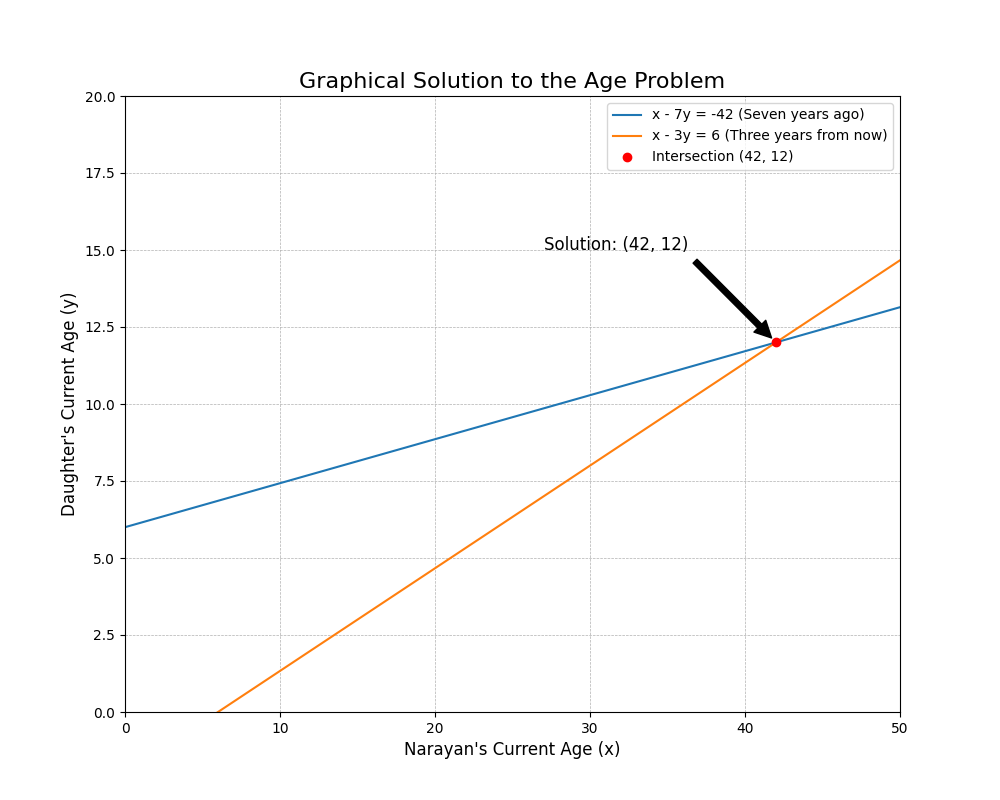
\includegraphics[width=0.85\columnwidth]{figs/graph12.png}
    \caption{5.8.10}
    \label{fig:placeholder}
\end{figure}
\end{document}